\chapter{Non-linear Static Structural - Strategies and Solutions} % Main chapter title

\label{Chapter2 } % For referencing the chapter elsewhere, use \ref{Chapter1} 
% \setlength{\parskip}{0.38cm}
\label{sec:nonlinear}
\vspace{0.38cm}
\newline
With geometrical non-linearity, alterations regarding geometrically linear observation:
\begin{itemize}
    \item Consideration of non-linear terms of the strain tensor E (kinematics)
     \item Establishing the forces equilibrium or application of the impulse theorem in the deformed
configuration (kinetics)

\end{itemize}
We use: 


\begin{itemize}
    \item  (Total) Lagrange point of view which is also described as the material point of view
     \item Stress and strain quantities in the undeformed configuration (second Piola Kirchhoff
stress tensor and Green Lagrange strain tensor)

\end{itemize}

The revolving point of this chapter is the numerical solution of non-linear vector equations $r_i(u)=r$ of time-independent structural mechanics as well as the assessment of deformation statesregarding the stability of the structure involved, as part of a geometrically non-linear finite
element analysis.
\newpage


\section{Kinematics}
\begin{figure}[h]
    \centering
    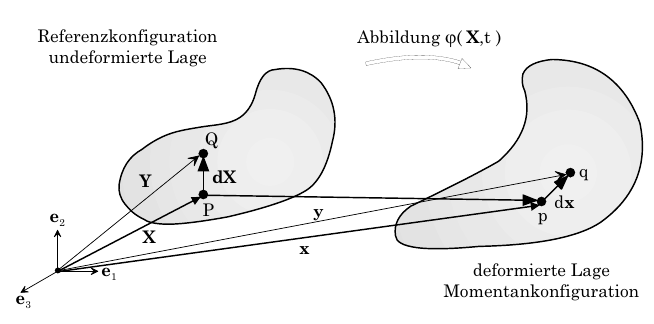
\includegraphics[scale=0.5]{Figures/Chapter2/anh3.png}
    \decoRule   
    \caption{ Current and reference configuration of a deformable material body}
    \label{fig:chap2anh3}
\end{figure}

\noindent
The fundamental of the geometrically non-linear formulation of structural mechanics is based on
the material deformation gradient F , which was already used within the scope of deriving the linear strain tensor  with the help of a non-linear deformation analysis of a material body, and
within the scope of subsequent linearization but not elaborated
because in linear observations it possesses no further significance. Non-linear observations are
a different story where the material deformation gradient defines the transformation from
reference to current configuration or from undeformed to deformed state and vice versa. These
transformations are referred to in technical literature as push forward and pull back. The
material deformation gradient is defined by a transformation of a line element dX of the
reference configuration to the current configuration dx (see figure \ref{fig:chap2anh3} ).

\begin{equation}
    dx = F \cdot dX; \quad F = \frac{{\partial x}}{{\partial X}} = \nabla x
\end{equation}
The Green Lagrange strain tensor E was also already derived and is given in equation (1.12) as function of the displacement gradient $\nabla u$ and its transpose ${\nabla ^T}u$. If we describe the
motion of the material point from the reference to the current configuration with help of the
displacement vector $\bf x = X + u$, the Green Lagrange strain tensor
\begin{equation}
    \label{5.7}
    E = \frac{1}{2}\left[ {{F^T} \cdot F - {\bf{1}}} \right] = {\nabla ^{{\rm{sym}}}}u + \frac{1}{2}{\nabla ^T}u \cdot \nabla u = \frac{1}{2}\left[ {{\nabla ^T}u + \nabla u + {\nabla ^T}u \cdot \nabla u} \right]
\end{equation}
can be represented as a function of the material deformation gradient.
\begin{equation}
 \boldsymbol{F}=\frac{\partial}{\partial \boldsymbol{X}}(\boldsymbol{X}+\boldsymbol{u})=\mathbf{1}+\nabla \boldsymbol{u} 
\end{equation}
According to this relation, the components of the term
\begin{equation}
 \nabla^{\operatorname{sym}} \boldsymbol{u}=\left[\begin{array}{ccc}u_{1,1} & \frac{1}{2}\left(u_{1,2}+u_{2,1}\right) & \frac{1}{2}\left(u_{1,3}+u_{3,1}\right) \\ \frac{1}{2}\left(u_{1,2}+u_{2,1}\right) & u_{2,2} & \frac{1}{2}\left(u_{2,3}+u_{3,2}\right) \\ \frac{1}{2}\left(u_{1,3}+u_{3,1}\right) & \frac{1}{2}\left(u_{2,3}+u_{3,2}\right) & u_{3,3}\end{array}\right] 
\end{equation}
of the linear part of the strain tensor E, given explicitly in equations (1.13) and (1.14), are
supplemented by the term $1/2 \nabla^T u$ · $\nabla u$, in the scope of geometrically non-linear theory, which can again be calculated with the displacement vector gradient according to eq. (1.7)
\begin{equation}
 \nabla \boldsymbol{u}=\left[\begin{array}{lll}u_{1,1} & u_{1,2} & u_{1,3} \\ u_{2,1} & u_{2,2} & u_{2,3} \\ u_{3,1} & u_{3,2} & u_{3,3}\end{array}\right] 
\end{equation}
by matrix multiplication.
\begin{equation}
 \frac{1}{2} \nabla^{T} \boldsymbol{u} \cdot \nabla \boldsymbol{u}=\frac{1}{2}\left[\begin{array}{lll}u_{k, 1}u_{k, 1} & u_{k, 1}u_{k, 2} & u_{k, 1} u_{k, 3} \\ u_{k, 2}u_{k, 1} & u_{k, 2}u_{k, 2} & u_{k, 2}u_{k, 3} \\ u_{k, 3}u_{k, 1} & u_{k, 3}u_{k, 2} & u_{k, 3}u_{k, 3}\end{array}\right] 
\end{equation}
It should be noted that the summation is performed over $k = 1, 2, 3$, respectively. The component presentation of the Green Lagrange strain tensor finally yields the following:
\begin{equation}
\label{5.12}
 E_{i j}=\frac{1}{2}\left(u_{i, j}+u_{j, i}+u_{k, i} u_{k, j}\right); \qquad \boldsymbol{E}=E_{i j} \boldsymbol{E}_{i} \otimes \boldsymbol{E}_{j} 
\end{equation}
In order to formulate the non-linear Finite Element methods, it remains to convert the calculation rule of the strain tensor, given in eq. (\ref{5.7}) or (\ref{5.12}), into the calculation rule of the strain
vector in a suitable way . The linear part of the strain tensor can be expressed as a vector by
application of the differential operator $D_\varepsilon$ to the displacement vector u, as described in eq.
(1.16). However, for the non-linear part of the strain tensor, no suitable operator presentation
can be found.
\begin{equation}
\label{5.13}
    {\bf{E}}({\bf{u}}) = \left[ {\begin{array}{*{20}{c}}
{{E_{11}}}\\
{{E_{22}}}\\
{{E_{33}}}\\
{2{E_{12}}}\\
{2{E_{23}}}\\
{2{E_{13}}}
\end{array}} \right] = \left[ {\begin{array}{*{20}{c}}
{{u_{1,1}}}\\
{{u_{2,2}}}\\
{{u_{3,3}}}\\
{{u_{1,2}} + {u_{2,1}}}\\
{{u_{2,3}} + {u_{3,2}}}\\
{{u_{1,3}} + {u_{3,1}}}
\end{array}} \right] + \left[ {\begin{array}{*{20}{l}}
{1/2\left( {{u_{1,1}}{u_{1,1}} + {u_{2,1}}{u_{2,1}} + {u_{3,1}}{u_{3,1}}} \right)}\\
{1/2\left( {{u_{1,2}}{u_{1,2}} + {u_{2,2}}{u_{2,2}} + {u_{3,2}}{u_{3,2}}} \right)}\\
{1/2\left( {{u_{1,3}}{u_{1,3}} + {u_{2,3}}{u_{2,3}} + {u_{3,3}}{u_{3,3}}} \right)}\\
{{u_{1,1}}{u_{1,2}} + {u_{2,1}}{u_{2,2}} + {u_{3,1}}{u_{3,2}}}\\
{{u_{1,2}}{u_{1,3}} + {u_{2,2}}{u_{2,3}} + {u_{3,2}}{u_{3,3}}}\\
{{u_{1,1}}{u_{1,3}} + {u_{2,1}}{u_{2,3}} + {u_{3,1}}{u_{3,3}}}
\end{array}} \right]{\rm{ }}
\end{equation}
According to eq (\ref{5.13}), the Green Lagrange strain tensor of geometrically non-linear
deformations is obtained by addition of the well-known linear part ${\bf D}_\varepsilon \bf u$ and the non-linear part $\bf E^\textnormal{nl}(u)$,
\begin{equation}
 \boldsymbol{E}(\boldsymbol{u})=\mathbf{D}_{\varepsilon} \boldsymbol{u}+\boldsymbol{E}^{n l}(\boldsymbol{u}) 
\end{equation}
where  ${\bf D}_\varepsilon \bf u$ and $\bf E^\textnormal{nl}(u)$ are defined as follows (summation over $k = 1, 2, 3$).

\begin{equation}
    {{\bf{D}}_\varepsilon }{\bf{u}} = \left[ {\begin{array}{*{20}{c}}
{{u_{1,1}}}\\
{{u_{2,2}}}\\
{{u_{3,3}}}\\
{{u_{1,2}} + {u_{2,1}}}\\
{{u_{2,3}} + {u_{3,2}}}\\
{{u_{1,3}} + {u_{3,1}}}
\end{array}} \right]\qquad {{\bf{E}}^{nl}}({\bf{u}}) = \left[ {\begin{array}{*{20}{l}}
{1/2}{{u_{k,1}}}{{u_{k,1}}}\\
{1/2}{{u_{k,2}}}{{u_{k,2}}}\\
{1/2}{{u_{k,3}}}{{u_{k,3}}}\\
{{u_{k,1}}}{{u_{k,2}}}{}\\
{{u_{k,2}}}{{u_{k,3}}}{}\\
{{u_{k,1}}}{{u_{k,3}}}{}
\end{array}} \right]
\end{equation}

\section{Kinetics}

Unlike the linear structural analysis, its non-linear counterpart requires that the dynamic or
the static forces equilibrium be observed in the deformed configuration. This firstly calls for
the evaluation of mass distribution which gives the relation between density in the current
configuration $\rho_c$ and the one in the reference configuration $\rho$, with the help of determinant $|F|$ of the material deformation gradient
\begin{equation}
 \rho=|\boldsymbol{F}| \rho_{c} 
 \label{eqn:5.18} 
\end{equation}

The forces equilibrium of a geometrically linear approximation, was obtained by pure kinetic analysis of a differential volume element. Analoguous analysis of a volume element in a deformed configuration gives us the \textsc{Cauchy} motion equation in the so called spatial or \textsc{Euler} formulation.
\begin{equation}
 \rho_{c} \ddot{u}=\operatorname{div} \sigma+\rho_{c} b \quad \forall \quad x \in \Omega 
 \label{eqn:5.19} 
\end{equation}
$\operatorname{div} \sigma$ symbolises the tensor divergence of the real stresses or the Cauchy stress tensor, related
to the current configuration. As the first description of this stress tensor might lead us to anticipate, this stress quantity is defined by a differential load in the current configuration, effecting
a deformed surface element $da$, arbitrarily oriented with a normal vector $\bf n$ inside the body,
leading to the consequence that the actual stresses occurring in the material can be described.

It is of advantage to numerical conversion in structural mechanics to utilize the motion equation in the materialor Lagrange formulation. To perform this it is necessary to relate the Cauchy
motion equation to the undeformed configuration. Multiplication of motion equation (\ref{eqn:5.19})
by determinant of the material deformation gradient already transforms the density in the
reference configuration, according to (\ref{eqn:5.18}).

\begin{equation}
 \begin{array}{ll}|\boldsymbol{F}| \rho_{c} \ddot{\boldsymbol{u}}=|\boldsymbol{F}| \operatorname{div} \boldsymbol{\sigma}+|\boldsymbol{F}| \rho_{c} \boldsymbol{b} & \rho \ddot{\boldsymbol{u}}=|\boldsymbol{F}| \operatorname{div} \boldsymbol{\sigma}+\rho \boldsymbol{b}\end{array} 
 \label{eqn:5.20} 
\end{equation}

It remains to transform the middle term of the equation. Since this transformation requires the
profound familiarity with non-linear continuum mechanics, we shall leave out the derivation
procedure and resort to the related literature for the result. To clarify the outcome,we shall give the resulting identity in symbolic presentation and it component notation.
\begin{equation}
 |\boldsymbol{F}| \operatorname{div} \boldsymbol{\sigma}=\operatorname{DIV}(\boldsymbol{F} \cdot \boldsymbol{S}) \quad|\boldsymbol{F}| \frac{\partial \sigma_{i j}}{\partial x_{j}}=\frac{\partial\left(F_{i k} S_{k j}\right)}{\partial X_{j}} 
 \label{eqn:5.21} 
\end{equation}

$DIV$ symbolises the divergence operator with respect to the reference configuration. Tensor
$S$, which is here used for the first time, is the second \textbf{{Piola Kirchhoff}} stress tensor defined with respect to the reference configuration. It should be noted that the Piola Kirchhoff stress
tensor $S$, unlike the Cauchy stress tensor $\sigma$, does not refer to actual stresses but to ’pseudo
stresses’. They are defined with respect to the reference configuration by a differential load
effecting a surface element of the reference configuration $dA$, which is oriented with a normal
vector $N$ . Introduction of equation (\ref{eqn:5.21}) into equation (\ref{eqn:5.20}) eventually yields the material or the Lagrange formulation of impulse rule, that is, the \textsc{Cauchy} motion equation.
\begin{equation}
 \rho \ddot{\boldsymbol{u}}=\operatorname{DIV}(\boldsymbol{F} \cdot \boldsymbol{S})+\rho \boldsymbol{b} \quad \forall \quad \boldsymbol{X} \in \Omega 
 \label{eqn:5.22} 
\end{equation}

In order to formulate a well-defined problem, it is necessary to supplement the impulse rule
with the static or \textsc{Neumann} boundary condition.  It is possible to apply the procedure for derivation of equilibrium
at the boundary, demonstrated in the geometrically linear case, to the deformed configuration
\begin{equation}
 \begin{array}{ccc}\sigma \cdot n=t^{\star} & \forall & x \in \Gamma_{\sigma}\end{array} 
 \label{eqn:5.23} 
\end{equation}
and thereupon to transform it. Material formulation of the Neumann boundary conditions is
in the geometrically non-linear case defined by
\begin{equation}
 \boldsymbol{F} \cdot \boldsymbol{S} \cdot \boldsymbol{N}=\boldsymbol{T}^{\star} \quad \forall \quad \boldsymbol{X} \in \Gamma_{\sigma} 
 \label{eqn:5.24} 
\end{equation}
where N presents the normal vector of reference
configuration. Stress vector $T$ (first Piola Kirchhoff stress tensor) is defined by a differential
load vector of current configuration acting on a surface element of the reference configuration
$dA$ parallel to $t^*$  .
\begin{equation}
 \boldsymbol{T}^{\star} d A=\boldsymbol{t}^{\star} d a 
 \label{eqn:5.23} 
\end{equation}

%-----------------------------------------------------
\section{Hyperelastic Materials \parencite{medium} \parencite{ref4}}
In structural finite element analysis, non-metal materials such as rubber and biological tissues are often encountered. Because the mechanical properties of these materials are very different from the mechanical properties of metal materials, such as large elastic deformation, incompressibility, viscoelasticity, etc. Researchers and engineers classify these materials as hyperelastic materials, and group the mechanical models that describe such materials as hyperelastic models.
\begin{figure}[H]
    \centering
    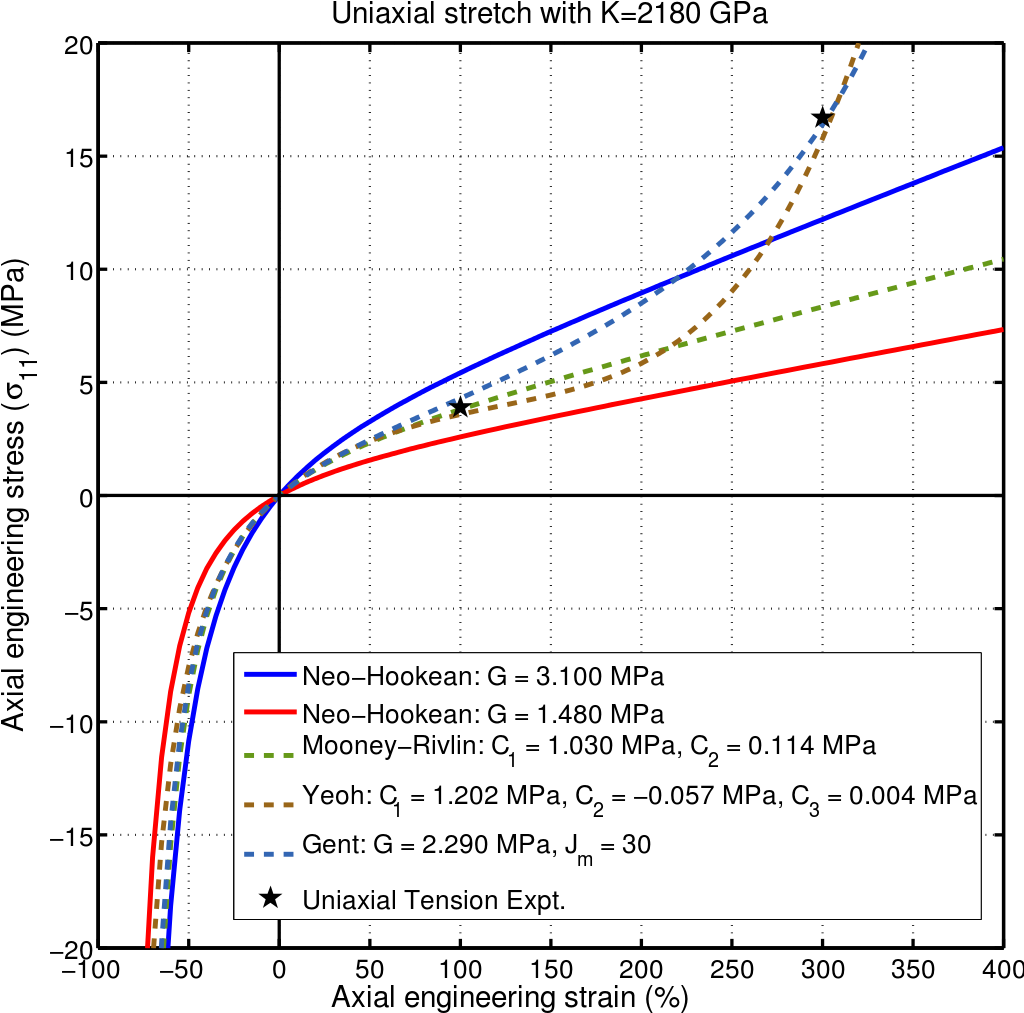
\includegraphics[scale=0.35]{Figure2/Chap3/diffhyper.png}
    \caption{The difference between elastic and hyperelastic materials in stress-strain relationship}
    \label{fig:my_label}
\end{figure}

Material behavior is described by its constitutive
relation when subjected to deformation or deformation history. Different constitutive relations can represent different material behaviors. The St. Venant–Kirchhoff
material provides a linear relation between stress and strain, which is a
simple extension of the one used for linear elastic materials. Unfortunately, this
model provides meaningful results only when the strains are small because most
materials show a nonlinear relation for large deformation. It is important to employ
a constitutive model that is appropriate for the material, the structure, and the finite
element formulation.

When the material status can completely be describable with a given total strain,
the constitutive relation is called hyperelasticity. In such a material, a strain energy density exists as a function of strain, and stress can be obtained by differentiating
the strain energy density with respect to strain. This material model is independent
of deformation history; i.e., the same deformation is expected if the final load is the
same. Rubberlike materials or human tissues belong in this category. On the other
hand, when the constitutive relation is given in terms of the stress and strain rates, it
is called hypoelasticity, which is often used in describing the plastic behavior of
materials. In such a material, the deformation history must be followed to calculate
stress because two states that have the same strain may have different stresses
depending on the loading history. Hyperelastic materials will be discussed in this
section, while hypoelastic materials will be discussed in Chap. 4. In this section, the
static response of hyperelastic materials is formulated based on the material
description, i.e., the total Lagrangian formulation. Different hyperelastic materials
will be introduced, but the main development will be explained using the Mooney-
Rivlin material, which is the most popular material model. In general, hyperelastic
materials exhibit the property of being incompressible during finite deformation;
i.e., the volume of the material is preserved. This is a common behavior of many
elastic materials in finite deformation. Numerically, a constraint, $J = 1$, needs to be
imposed to make the material incompressible. However, this causes numerical
difficulties called volumetric locking. Due to incompressibility, the hydrostatic
portion of stress cannot be calculated from the volumetric strain. The penalty
method , the selective reduced integration method , and the mixed formula-
tion method have been successfully used for incompressible and nearly
incompressible materials.

If a strain energy density exists, such that stress can be obtained from the
derivative of the strain energy with respect to strain, the system is called path
independent. Thus, it is theoretically possible to solve the nonlinear equilibrium
equation for the given total magnitude of applied load. However, this equation is
still solved by using the incremental force method with a number of load steps to
finally reach the total applied load for computational purposes. The hyperelasticity
problem contains both material nonlinearity from constitutive relations and geometric nonlinearity from kinematics.

These hyperelastic materials (models) have the following significant characteristics:
\begin{itemize}
    \item Can withstand large elastic (recoverable) deformation, sometimes with stretch up to $1000\%$.
    \item Hyperelastic materials are almost incompressible. Because the deformation is caused by the straightening of the molecular chain of the material, the volume change under the applied stress is small.
    \item The stress-strain relationship is highly nonlinear. Normally, the material softens first and then hardens under tension, but hardens sharply when compressed.
\end{itemize}
%-------------------------------------
\subsection{Strain Energy Density}
Modeling engineering materials at large deformations is still an active research
area. Without elaborating details of material modeling procedures, a method that
can describe the behavior of isotropic elastic materials which undergo finite defor-
mation is presented. In hyperelasticity, the stored strain energy density is used to
compute stress. For isotropic materials, the constitutive relation has to be indepen-
dent of the coordinate frame selected because the material has the same property for
all directions. For example, the strain component E 11 cannot be used for the
constitutive relation because its value depends on the coordinate system. Thus, it
is natural that the strain energy density is defined using invariants of strain or
alternatively that of the deformation tensor. When the undeformed state is used as
the frame of reference, the three invariants of the right Cauchy–Green deformation
tensor $C$ are given as

\begin{equation}
 I_{1}=\operatorname{tr}(\mathbf{C})=\lambda_{1}^{2}+\lambda_{2}^{2}+\lambda_{3}^{2} 
     \label{eqn:3.101}
 \end{equation}
 \begin{equation}
 \label{eqn:3.102}
 I_{2}=\frac{1}{2}\left[(\operatorname{tr} \mathbf{C})^{2}-\operatorname{tr}\left(\mathbf{C}^{2}\right)\right]=\lambda_{1}^{2} \lambda_{2}^{2}+\lambda_{2}^{2} \lambda_{3}^{2}+\lambda_{3}^{2} \lambda_{1}^{2} 
\end{equation}
and
\begin{equation}
\label{eqn:3.103}
 I_{3}=\operatorname{det} \mathbf{C}=\lambda_{1}^{2} \lambda_{2}^{2} \lambda_{3}^{2} 
\end{equation}
where $ \lambda_{1}^{2}, \lambda_{2}^{2} $, and $ \lambda_{3}^{2} $ are three eigenvalues of the right Cauchy-Green deformation tensor C. From polar decomposition, it has been shown that $ \lambda_{1}, \lambda_{2} $, and $ \lambda_{3} $ are three eigenvalues of the left stretch tensor $ \mathbf{U}- $ also called the principal stretches. The above three invariants will remain unchanged for different coordinate systems. In order to be a valid deformation, the three invariants must be positive (refer to Example 3.1). The square root of $ I_{3} $ in Eq. (\ref{eqn:3.103}) measures the volume change of the material. If the material is incompressible, it is clear that $ I_{3}=1 $. The three invariants are identical for both the left and right Cauchy-Green deformation tensors. When there is no deformation, i.e., $ \lambda_{1}=\lambda_{2}=\lambda_{3}=1, I_{1}=I_{2}=3 $, and $ I_{3}=1 $.

\textit{Example}: (Invariants) Show that the three invariants of the left Cauchy-Green deformation tensor $ \mathbf{b} $ are equal to those of $ \mathbf{C} $ when the three eigenvalues of the deformation gradient are $ \lambda_{1}, \lambda_{2} $, and $ \lambda_{3} $.



Solution The three invariants will remain constant for different coordinate systems. Thus, it is possible to choose the three principal directions of the deformation gradient as basis vectors for the new coordinate system $ X^{\prime} Y^{\prime} Z^{\prime} $ so that the deformation gradient will only have diagonal components:
\begin{equation*}
 \mathbf{F}_{X^{\prime} Y^{\prime} Z^{\prime}}=\left[\begin{array}{ccc}\lambda_{1} & 0 & 0 \\ 0 & \lambda_{2} & 0 \\ 0 & 0 & \lambda_{3}\end{array}\right] 
\end{equation*}

Then the right and left Cauchy-Green deformation tensors become identical

\begin{equation}
 \mathbf{C}_{X^{\prime} Y^{\prime} Z^{\prime}}=\left(\mathbf{F}^{\mathrm{T}} \mathbf{F}\right)_{X^{\prime} Y^{\prime} Z^{\prime}}=\left[\begin{array}{ccc}\lambda_{1}^{2} & 0 & 0 \\ 0 & \lambda_{2}^{2} & 0 \\ 0 & 0 & \lambda_{3}^{3}\end{array}\right], \mathbf{b}_{X^{\prime} Y^{\prime} Z^{\prime}}=\left(\mathbf{F} \mathbf{F}^{\mathrm{T}}\right)_{X^{\prime} Y^{\prime} Z^{\prime}}=\left[\begin{array}{ccc}\lambda_{1}^{2} & 0 & 0 \\ 0 & \lambda_{2}^{2} & 0 \\ 0 & 0 & \lambda_{3}^{2}\end{array}\right] 
\end{equation}
and the three invariants of the two tensors are identical.


Using the three invariants, a general form of strain energy density can be defined in the following polynomials:
\begin{equation}
\label{eqn:3.104}
 W\left(I_{1}, I_{2}, I_{3}\right)=\sum_{m+n+k=1}^{\infty} A_{m n k}\left(I_{1}-3\right)^{m}\left(I_{2}-3\right)^{n}\left(I_{3}-1\right)^{k} 
\end{equation}
where $ A_{m n k} $ are coefficients of polynomials. In general, deformation of a material can be decomposed into volumetric and distortional parts. If the material is incompressible, i.e., $ I_{3}=1 $, then the volumetric part of the strain energy density is eliminated, and only the first two terms contribute to the strain energy density. This part of the stored energy is called the distortional strain energy density and is defined as
\begin{equation}
\label{eqn:3.105}
W_{1}\left(I_{1}, I_{2}\right)=\sum_{m+n=1}^{\infty} A_{m n}\left(I_{1}-3\right)^{m}\left(I_{2}-3\right)^{n}
\end{equation}

Note that Eq. (\ref{eqn:3.105}) does not impose the incompressibility condition. A separate constraint must be used to make the material incompressible. All the models listed above account for nonconstant shear modulus. However, caution needs to be exercised on inclusion of higher-order terms to fit the data, since this may result in unstable energy functions, yielding nonphysical results outside the range of the experimental data. Various hyperelastic material models are proposed using Eq. (\ref{eqn:3.105}). 
%----------------------------------------
\subsection{Neo-Hookean Model }
Proposed by Ronald Rivlin (1915–2005) in 1948, Dr. Rivlin is also well-known for the Mooney-Rivlin hyper-elastic model. It can be seen that neo-Hookean is not a model named after a person. This British-American physicist studied physics and mathematics at St John’s College, Cambridge, being awarded a BA in 1937 and a ScD in 1952. He worked for the General Electric Company, then the UK Ministry of Aircraft Production, then the British Rubber Producers Research Association. He later moved to the United States and taught at Brown University and Lehigh University.

The Neo-Hookean model is the simplest form of all commonly used hyper-elastic models. This model has only one nonzero parameter, $ A_{10} $, and all other parameters are zero. Using the undeformed state as a frame of reference, the strain energy density can be defined as
\begin{equation}
\label{eqn:3.106}
 W_{1}\left(I_{1}\right)=A_{10}\left(I_{1}-3\right) 
\end{equation}

In order to be equivalent to the linear elastic material in small deformation, the parameter $ A_{10} $ is related to the shear modulus by $ A_{10}=\mu / 2 $. The stress-strain relation becomes linear with a proportional constant of $ 2 A_{10}=\mu $. However, this model will show a nonlinear relationship when the deformation becomes larger due to the nonlinear displacement-strain relation. This model gives a good correlation with the experimental data up to $ 40 \% $ strain in uniaxial tension and up to $ 90 \% $ strains in simple shear. This model is often used to describe the behavior of crosslinked polymers.

Although this model is not as versatile as other models, especially for large strain or tensile conditions. The neo-Hookean model has the following advantages:
\begin{enumerate}
    \item  \textbf{Simple}. There are only 2 input parameters. If the material is assumed to be incompressible, then only one parameter is required: the initial shear modulus. Since only one parameter is needed from the test data, the number of required tests is small.
    \item \textbf{Compatible}. The material parameter obtained from one type of deformation stress-strain curve can be used to predict other types of deformation. Especially for the small and medium strain conditions.
\end{enumerate}

It is worth mentioning that neo-Hookean is not only applied to science and engineering but also used in the computer graphics in the filming industry because of its simplicity and physical-based solutions. For example, the process of hand movement, the muscle and skin changes calculated using the neo-Hookean model appear extremely natural.

\subsection{Example for Neo-Hookean Model}
We discuss the stress–strain relationship for Neo–Hookean model in example below:
\textit{Example:} Plot the nominal stress–strain relationship for a Neo–Hookean model under uniaxial tension and
compression and compare it with linear elastic material with the same modulus.
Assume material parameter A 10  10MPa and incompressibility.

\textit{Solution:} Let us suppose that a uniaxial load is stretched so that $\lambda_ 1  \lambda$ where $ \lambda $ is an
arbitrary stretch along the rod’s length. From the assumption of incompressibility,
$\lambda_ 1 \lambda _2 \lambda_ 3  =1 $ and $ \lambda_ 2  \lambda_3$ . Therefore,$ \lambda_ 2  \lambda _3  =1/ \lambda$ . From Eq. (\ref{eqn:3.106}), the strain energy density of the Neo–Hookean material model becomes
\begin{equation*}
 W=A_{10}\left(I_{1}-3\right)=A_{10}\left(\lambda_{1}^{2}+\lambda_{2}^{2}+\lambda_{3}^{2}-3\right)=A_{10}\left(\lambda^{2}+\frac{2}{\lambda}-3\right) 
\end{equation*}
\input{Page/Chap3/Hyperlastic Material/5}
The nominal stress (first Piola-Kirchhoff stress) in the direction of stretch can be obtained by differentiating the strain energy density with respect to the principal stretch as

$ P=\frac{\partial W}{\partial \lambda}=2 A_{10}\left(\lambda-\frac{1}{\lambda^{2}}\right)=\mu\left(1+\varepsilon-\frac{1}{(1+\varepsilon)^{2}}\right) $

Figure $ \ref{fig:3.13} $ shows the stress-strain curve for the Neo-Hookean material, along with a linear elastic material. Since Poisson's ratio for the incompressible material is $ 0.5 $, Young's modulus will be $ E=3 \mu $. Both curves share the same tangent line at $ \varepsilon=0 $, but the error increases as the strain increases. One thing to note is that the NeoHookean model shows a quite different behavior in compression from the linear elastic material behavior.

\begin{figure}[H]
    \centering
    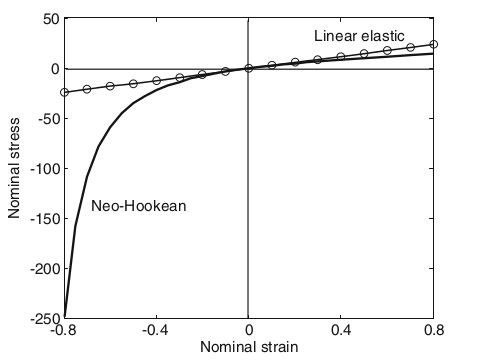
\includegraphics[scale=0.7]{Figure2/Chap3/neohk.png}
    \caption{Stress–strain relationship for Neo–Hookean material in example}
    \label{fig:3.13}
\end{figure}


\subsection{Nearly Incompressible Hyperelasticity}
Incompressibility of a material can cause many difficulties in the constitutive
relation, especially when it is combined with nonlinearities such as large displace-
ments, large strains, and contact. Perfect incompressibility, which corresponds to
Poisson’s ratio of one-half, is an idealization to make modeling more amenable for
obtaining closed-form solutions. In the real world, natural as well as filled rubbers
are slightly compressible, thereby, facilitating development of algorithms for nearly
incompressible behavior of elastomers. “Near-incompressibility” means that
Poisson’s ratio is not exactly one-half, but close to it. For example, 0.49 or higher
values are often used for the nearly incompressible behavior of elastomers.

As discussed previously, the hydrostatic pressure portion of stress causes volume
change (dilatation). However, if the material is incompressible, the volume remains
constant for different values of pressure. In other words, stress cannot be obtained
by differentiating the strain energy density because the hydrostatic pressure portion
of stress cannot be determined from deformation.

It has been observed from experiments that many rubberlike materials show
nearly incompressible properties. It means that only a small volume change occurs
under a large hydrostatic pressure. In such materials, the near-incompressibility can
be imposed by using a large bulk modulus, which relates hydrostatic pressure to
volumetric strain. Since the material is stiff in dilatation and soft in distortion, it is
necessary to separate these two parts in order to reduce numerical difficulties
associated with a large difference in stiffness. This has to be done in the level of
strain energy density.

In the previous section, it is discussed that the third invariant $I _3$ is related to
dilatation, while the other two invariants, $I_ 1$ and $I _2$ , are related to distortion.
However, $I _1$ and $I _2$ do not remain constant during dilatation
In order to separate the distortion part from dilatation, it is necessary to introduce the so-called reduced invariants, $ J_{1}, J_{2} $, and $ J_{3} $, defined by
\begin{equation}
 J_{1}=I_{1} I_{3}^{-1 / 3}, \quad J_{2}=I_{2} I_{3}^{-2 / 3}, \quad J_{3}=I_{3}^{1 / 2} 
\end{equation}
where $ I_{1}, I_{2} $, and $ I_{3} $ are the three invariants of the right Cauchy-Green deformation tensor C. It can be easily verified that $ J_{1} $ and $ J_{2} $ are constant under pure dilatation; they are only related to distortion, while $ J_{3} $ is related to dilatation. Of course, when the material is purely incompressible, the reduced invariants are the same with the invariants of $ \mathbf{C} $.

Using the reduced invariants, it is possible to separate the distortion effect from dilatation in defining the strain energy density, as
\begin{equation}
 W\left(J_{1}, J_{2}, J_{3}\right)=W_{1}\left(J_{1}, J_{2}\right)+W_{2}\left(J_{3}\right) 
\end{equation}
where $ W_{1}\left(J_{1}, J_{2}\right) $ is the distortional strain energy density and $ W_{2}\left(J_{3}\right) $ is the dilatational strain energy density. The distortional energy density can be defined using Eq. (\ref{eqn:3.105}) by substituting the reduced invariants for the original invariants. An example of the dilatational energy density is related to the bulk modulus of the material as
\begin{equation}
W_{2}\left(J_{3}\right)=\frac{K}{2}\left(J_{3}-1\right)^{2}
\end{equation}

where $ K $ is the bulk modulus. The relationship between the bulk modulus and Lame's constants for an isotropic material can be written as
\begin{equation}
K=\lambda+\frac{2}{3} \mu
\end{equation}

The above relation is valid for linear elastic materials. For general nearly incompressible materials, a large value of the bulk modulus is used-two or three orders of magnitude larger than material parameters in the distortional part. The material becomes incompressible as the bulk modulus approaches infinity.

\subsection{ Algorithm for Stress Calculation}

In computer programming, it is convenient to use vector and matrix notation rather than tensor notation. Thus, in the following algorithm, vector and matrix notation will be used. Below is the procedure of stress calculation for the Mooney-Rivlin hyperelastic material. The inputs are the Lagrangian strain and material parameters, and the outputs are the six components of the second Piola-Kirchhoff stress:

\begin{enumerate}
\item For given strain $ \{\mathbf{E}\}=\left\{E_{11}, E_{22}, E_{33}, E_{12}, E_{23}, E_{13}\right\}^{\mathrm{T}} $ and given material

constants $ \left(A_{10}, A_{01}\right. $, and $ K $ ) for the penalty method, or material constants $ \left(A_{10}\right. $ and $ A_{01} $ ) and the hydrostatic pressure $ p $ for the mixed formulation method, perform the following calculation.

\item  Set $ \{\mathbf{1}\}=\{1,1,1,0,0,0\}^{\mathrm{T}} $ and $ \{\mathbf{C}\}=2 \times\{\mathbf{E}\}+\{\mathbf{1}\} $.

\item  Calculate the three invariants:

$I_1=C_1 + C_2 + C_3$

$ I_{2}=C_{1} \times C_{2}+C_{1} \times C_{3}+C_{2} \times C_{3}-C_{4} \times C_{4}-C_{5} \times C_{5}-C_{6} \times C_{6} $

$ I_{3}=\left(C_{1} \times C_{2}-C_{4} \times C_{4}\right) \times C_{3}+\left(C_{4} \times C_{6}-C_{1} \times C_{5}\right) \times C_{5}+ \\ \left(C_{4} \times C_{5}-C_{2} \times C_{6}\right) \times C_{6} $



\item Calculate the derivatives of invariants with respect to the Lagrangian strain:

$\left\{I_{1, \mathbf{E}}\right\}=2 \times \{1\}$

$ \left\{I_{2, \mathbf{E}}\right\}=2 \times\left\{C_{2}+C_{3}, C_{3}+C_{1}, C_{1}+C_{2},-C_{4},-C_{5},-C_{6}\right\}^{\mathrm{T}} $



$ \left\{I_{3, \mathbf{E}}\right\}=2 \times\left\{C_{2} C_{3}-C_{5} C_{5}, C_{3} C_{1}-C_{6} C_{6}, C_{1} C_{2}-C_{4} C_{4} - \right. $



$ \left.C_{5} C_{6}-C_{3} C_{4}, C_{6} C_{4}-C_{1} C_{5}, C_{4} C_{5}-C_{2} C_{6}\right\}^{\mathrm{T}} $



\item  Calculate the derivatives of the reduced invariants.



$ \left\{J_{1, \mathbf{E}}\right\}=I_{3}^{-1 / 3}\left\{I_{1, \mathbf{E}}\right\}-\frac{1}{3} I_{1} I_{3}^{-4 / 3}\left\{I_{3, \mathbf{E}}\right\} $

$ \left\{J_{2, \mathbf{E}}\right\}=I_{3}^{-2 / 3}\left\{I_{2, \mathbf{E}}\right\}-\frac{2}{3} I_{2} I_{3}^{-5 / 3}\left\{I_{3, \mathbf{E}}\right\} $



$ \left\{J_{3, \mathbf{E}}\right\}=\frac{1}{2} I_{3}^{-1 / 2}\left\{I_{3, \mathbf{E}}\right\} $



\item  Calculate the second Piola-Kirchhoff stress from Neo-Hookean model:

$ \{\mathbf{S}\}=A_{10}\left\{J_{1, \mathbf{E}}\right\}+A_{01}\left\{J_{2, \mathbf{E}}\right\}+p\left\{J_{3, \mathbf{E}}\right\} . $

When the penalty method is used, then use $ K\left(J_{3}-1\right) $ instead of $ p $.

\end{enumerate}




%--------------------------------------------------------
\section{Strategies for Non-linear static structural equations \parencite{Advance} }
\begin{figure}[H]
    \centering
    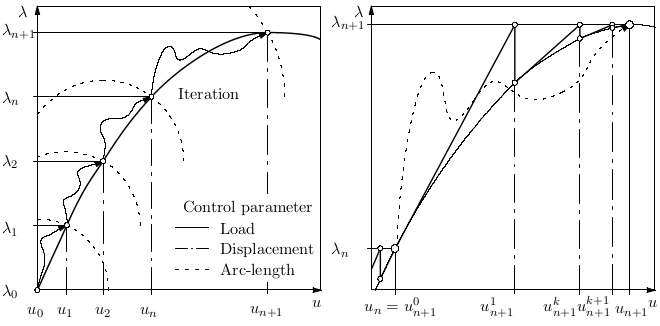
\includegraphics[scale=0.55]{Figure2/Chap3/local iteration.png}
    \caption{Load parameter control $(\lambda_n \rightarrow r_{in})$ and local iteration (Newton-Raphson)}
    \label{fig:7.1}
\end{figure}
We have non-linear vector equation
\begin{equation}
    \label{eqn:7.1} 
    r_i(u)=r
\end{equation}

The procedures for solving equation (\ref{eqn:7.1}) consist of two components:
\begin{itemize}
    \item The control methods or control procedures describe the successive load application.
    \item The iteration procedures serve the purpose of finding the equilibrium states for an incremental load change.
\end{itemize}
As shown in figure \ref{eqn:7.1}, the load application control is realized by controlling the load, the
displacement or the so called arc length along the equilibrium path which characterises the
equality of internal forces and external loads. The control of load application is accomplished
by parametrization of equation (\ref{eqn:7.1}) with the load factor $\lambda$
\begin{equation}
 \boldsymbol{r}_{i}(\boldsymbol{u})=\lambda \boldsymbol{r} \quad[0, \lambda]=\bigcup_{n=1}^{N T} \lambda_{n+1}-\lambda_{n} 
 \label{eqn:7.2} 
\end{equation}
where $\lambda$ is applied step-wise for the numerical transformation of the solution. The load steps induced in such a way are numbered in analogy with the time steps of transient problems, 
with $n = 1,\ldots, NT$ . The equilibrium state corresponding to the load factor \lambda n , is described with displacements $u_n$ . This explains why with the numerical solution of the non-linear
equation (7.1), only discrete supporting points of the path can be acquired, not the continuous
equilibrium path. The number, the separation, and the arrangement of supporting points
is determined by the control procedure which shall be derived in detail in chapter 7.3. The
step-wise numerical solution from one supporting point to the other is accomplished for example
by means of the pure Newton-Raphson method, the modified Newton-Raphson method
or the Quasi-Newton methods. Starting from an equilibrium state characterised by the
displacement state $u_n$ and the internal forces$ r _i (u_n ) $ calculable from that state, we numerically
compute the equilibrium point for the load factor $\lambda_{ n+1} $, by means of solution $(u_{n+1} , r_i (u_{n+1} ))$.
In figure 7.1, we see an example of the schematic presentation of equilibrium iteration of the
load-controlled pure Newton-Raphson procedure of a one-dimensional non-linear equation
$r_ i (u) = r$. The derivation and the numerical properties of this and the other methods are
discussed in chapter \ref{chap:7.2}.
%----------------------------------------------------------------------
\section{Iteration Methods}
\label{sec:7.2}
\label{chap:7.2}
All methods presented here are based on the multi-dimensional Taylor row expansion of the
internal forces vector at a deformation state determined by the structural displacement vector
$u ^k_{n+1}$
\begin{equation}
 r_{i}\left(\boldsymbol{u}_{n+1}^{k+1}\right)=\boldsymbol{r}_{i}\left(\boldsymbol{u}_{n+1}^{k}\right)+\frac{\partial \boldsymbol{r}_{i}\left(\boldsymbol{u}_{n+1}^{k}\right)}{\partial \boldsymbol{u}_{n+1}^{k}}\left(\boldsymbol{u}_{n+1}^{k+1}-\boldsymbol{u}_{n+1}^{k}\right)+\frac{1}{2} \frac{\partial^{2} \boldsymbol{r}_{i}\left(\boldsymbol{u}_{n+1}^{k}\right)}{\partial \boldsymbol{u}_{n+1}^{k 2}}\left(\boldsymbol{u}_{n+1}^{k+1}-\boldsymbol{u}_{n+1}^{k}\right)^{2}+\cdots 
 \label{eqn:7.3} 
\end{equation}

The result of a Taylor row is approximated by the vector of internal forces of the displacement
state $u^{k+1}_{n+1}$
n+1 in the neighbourhood of point $u^{k}_{n+1}$ . It should be noted that the index $k$, used to designate both neighbouring displacement states, stands for the iteration index in dealing with the
iteration procedure. To generate the iteration procedure, the Taylor row expansion is aborted
after the linear term and the difference of both displacement states is termed displacement increment $\Delta u = u^{k+1}_{n+1}-u^{k}_{n+1}$.
\begin{equation}
 \boldsymbol{r}_{i}\left(\boldsymbol{u}_{n+1}^{k+1}\right)=\boldsymbol{r}_{i}\left(\boldsymbol{u}_{n+1}^{k}\right)+\frac{\partial \boldsymbol{r}_{i}\left(\boldsymbol{u}_{n+1}^{k}\right)}{\partial \boldsymbol{u}_{n+1}^{k}} \Delta \boldsymbol{u} 
 \label{eqn:7.4} 
\end{equation}

The partial derivative of the system vector of internal forces with respect to the actual
displacement state $u^ k_{n+1}$ contained in this equation is the tangential stiffness matrix of this state
\begin{equation}
 \boldsymbol{r}_{i}\left(\boldsymbol{u}_{n+1}^{k+1}\right)=\boldsymbol{r}_{i}\left(\boldsymbol{u}_{n+1}^{k}\right)+\mathbf{K}_{t}\left(\boldsymbol{u}_{n+1}^{k}\right) \Delta \boldsymbol{u} \qquad \qquad \Delta \boldsymbol{u}=\boldsymbol{u}_{n+1}^{k+1}-\boldsymbol{u}_{n+1}^{k} 
\label{eqn:7.5} 
\end{equation}

 $K_t (u^ k_{n+1} \Delta u$ is identical to the linearization of the vector of
internal forces $\Delta r_i(u^k_{n+1})$, so that the equation (\ref{eqn:7.5}) can be interpreted as incremental change
of internal forces for an incremental change of the displacement state.
%--------------------------------------------------------------------
\subsection{Pure Newton-Raphson Method}
\noindent
\begin{figure}[H]
    \centering
    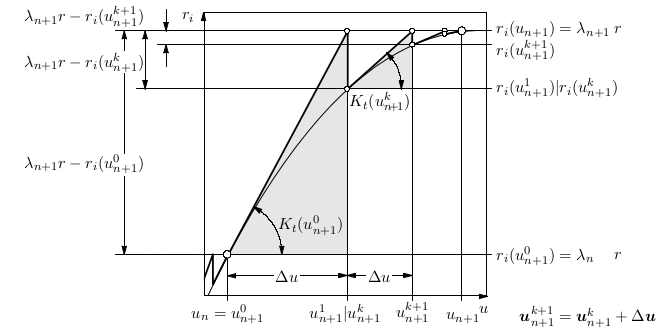
\includegraphics[scale=0.6]{Figure2/Chap3/Pure Newton-Raphson.png}
    \caption{Pure Newton-Raphson Iteration}
    \label{fig:7.2}
\end{figure}
The development of the vector of internal forces into a Taylor row according to equation (\ref{eqn:7.5}),
and the requirement for fulfilment of the equilibrium relation (\ref{eqn:7.2}), comprise the basis of the
Newton-Raphson method which was first published by Cauchy in 1847.
\begin{equation}
 \boldsymbol{r}_{i}\left(\boldsymbol{u}_{n+1}^{k+1}\right)=\boldsymbol{r}_{i}\left(\boldsymbol{u}_{n+1}^{k}\right)+\mathbf{K}_{t}\left(\boldsymbol{u}_{n+1}^{k}\right) \Delta \boldsymbol{u}=\lambda_{n+1} \boldsymbol{r} 
 \label{eqn:7.8} 
\end{equation}

In this context, the displacement increment $\Delta u$ is often denoted as the Newton correction. As
it will soon become clear, in the beginning of load step $n + 1$ we can set out from an equilibrium
state.
\begin{equation}
    r_i(u_n)=\lambda _nr
    \label{eqn:7.9}
\end{equation}

In order to locate the equilibrium for load factor $\lambda_{n+1}$ , we now demand that the approximation of internal forces of the deformation state $u_1^{n+1}$ , based on Taylor row expansion at the
development point $u_n=u^0_{n+1}$ , fulfils the equilibrium relation at the end of the load step.
\begin{equation}
 \boldsymbol{r}_{i}\left(\boldsymbol{u}_{n+1}^{1}\right)=\boldsymbol{r}_{i}\left(\boldsymbol{u}_{n+1}^{0}\right)+\mathbf{K}_{t}\left(\boldsymbol{u}_{n+1}^{0}\right) \Delta \boldsymbol{u}=\lambda_{n+1} \boldsymbol{r} 
 \label{eqn:7.10} 
\end{equation}

The solution of this equation yields the displacement increment, which gives the approximation
of solution $(u^1_{ n+1} )$ with equation (\ref{eqn:7.5}).
\begin{equation}
 \Delta \boldsymbol{u}=\mathbf{K}_{t}^{-1}\left(\boldsymbol{u}_{n+1}^{0}\right)\left(\lambda_{n+1} \boldsymbol{r}-\boldsymbol{r}_{i}\left(\boldsymbol{u}_{n+1}^{0}\right)\right) \quad \boldsymbol{u}_{n+1}^{1}=\boldsymbol{u}_{n+1}^{0}+\Delta \boldsymbol{u} 
 \label{eqn:7.11} 
\end{equation}

Generally, the first calculation step of an iteration method is termed predictor. The quality of
solution u 1 n+1 can be evaluated by means of the so called residuum $ \lambda_{n+1} r-\boldsymbol{r}_{i}\left(\boldsymbol{u}_{n+1}^{1}\right) $
. In the
case of equilibrium which is attainable only hypothetically, the residuum vanishes. In order to
close in on this hypothetical ideal case, we can repeat the procedure defined by equations (\ref{eqn:7.10})
and (\ref{eqn:7.11} for calculating the displacement vector $u^2_ {n+1} $ based on $u ^1_{ n+1}$ . The displacement
vector $u_{n+1}^{k+1}$
is generally calculated based on the approximated solution $u ^k_{n+1} $. The method
for iterative solution of the non-linear vector equation (\ref{eqn:7.2}) generated by this is the pure
Newton-Raphson procedure, or shortly Newton-Raphson method. The updating relation,
described as corrector, and the resulting improvement of the solution vector $ u ^{k+1}_{n+1}$ follow from
transformation of equation (\ref{eqn:7.8}), having in mind the definition of the displacement increment
$\Delta u$.
\begin{equation}
 \Delta \boldsymbol{u}=\mathbf{K}_{t}^{-1}\left(\boldsymbol{u}_{n+1}^{k}\right)\left(\lambda_{n+1} \boldsymbol{r}-\boldsymbol{r}_{i}\left(\boldsymbol{u}_{n+1}^{k}\right)\right) \qquad \boldsymbol{u}_{n+1}^{k+1}=\boldsymbol{u}_{n+1}^{k}+\Delta \boldsymbol{u} 
 \label{eqn:7.12} 
\end{equation}

The procedure of solution improvement according to (\ref{eqn:7.12}) is repeated until the equilibrium is
reached approximately (see figure \ref{fig:7.2}). Here it should be stressed that the exact equilibrium
cannot be reached. Since this is a vector-value problem, we generate a scalar-valued criterion, a so called convergence criterion in order to judge whether a sufficient accuracy of the equilibrium
approximation is reached.  If the criterion is fulfilled, (here, because of completeness of
derivations, as example the criterion
\begin{equation}
 \eta_{u}^{k+1}=\frac{\|\Delta \boldsymbol{u}\|}{\left\|\boldsymbol{u}_{n+1}^{k+1}-\boldsymbol{u}_{n}\right\|} \leq \eta_{u} 
\label{eqn:7.13} 
\end{equation}
is given as an example ($\eta$ u is given by the user) the solution $u^{k+1}_{n+1}$ is approximated accurately
enough and the next load step can be solved analogously.

The pure Newton-Raphson method has the following properties
\begin{itemize}
    \item The pure Newton-Raphson method converges to a solution if the start vector $u^0_{ n+1} $ is close enough to the solution.
    \item The pure Newton-Raphson method converges locally quadratic.
\end{itemize}

The condition for convergence of the Newton-Raphson method can be fulfilled by successive loading of the structure. If convergence is not reached, the load step must be smaller. We
can, for example, adapt the size of the load step based on the convergence behaviour, which guaranties the convergent pursuit of the equilibrium path within the
scope of a non-linear FEM analysis. It remains to clarify the notion of local quadratic convergence. Local means that the quadratic convergence is reached in the vicinity of solution, which
practically means in the last one to two steps. The convergence rate describes the number of
necessary iterations, the higher the convergence rate, the less iteration steps are needed to solve
the non-linear equilibrium. It can be determined by means of evolution of the displacement
increment. The convergence rate ... is defined by the following equation (see equation (\ref{eqn:7.13})).

If the displacement increment decreases by the square, we talk about a quadratic convergence.

With the pure Newton-Raphson method we have presented the standard tool of modern non-
linear FEM analysis. We can grade it as robust in connection with suitable procedures for load
parameter control. For solution of larger systems with a correspondingly higher number of DOF,
this method however has proven to be very computation-time-consuming, since in each iteration
step a linear equation system (\ref{eqn:7.12}) must be solved. In order to circumvent this equation solution, which often needs to be performed and on top of that is costly, methods were developed which
approximate the deformation-dependent tangential stiffness matrix or its inverse. One of these
methods is the modified Newton-Raphson method; an entire group of such methods comprise
the Quasi-Newton procedures.
%----------------------------------------------------------
\subsection{Modified Newton-Raphson Method}
\begin{figure}[H]
    \centering
    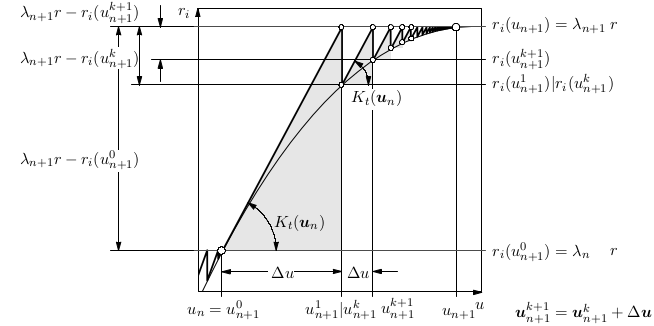
\includegraphics[scale=0.55]{Figure2/Chap3/Modified Newton-Raphson Iteration.png}
    \caption{Modified Newton-Raphson Iteration}
    \label{fig:7.3}
\end{figure}

The development of the modified Newton-Raphson method requires that we replace, in
equation (\ref{eqn:7.12}), the deformation-dependent tangential stiffness matrix, which therefore must be generated anew in each step, with the tangential stiffness matrix $K_t (u^ k_{n+1} )$ of the last known equilibrium state $K_t (u _n ) = K_t (u^0_{ n+1} )$ which is constant throughout the iteration.
\begin{equation}
 \Delta u=\mathbf{K}_{t}^{-1}\left(u_{n+1}^{0}\right)\left(\lambda_{n+1} r-r_{i}\left(u_{n+1}^{k}\right)\right) \qquad  \qquad u_{n+1}^{k+1}=u_{n+1}^{k}+\Delta u
 \label{eqn:7.14} 
\end{equation}
\section{Control of iteration procedures}
Now we must develop strategies for controlling the load
parameter $\lambda$. The latter globally controls the successive load increase, and, within the scope of
arc-length procedures and the displacement-controlled calculus, locally the applied external load
($\lambda n+1$ is altering with $k$).

The simplest possibility to control the loads acting on the system is the step-wise increase of the load with each load step $n$. This external load is constant during the equilibrium iteration which ensures the attainment of equilibrium state correlated to the corresponding load $\lambda_ {n+1}$ , after successful iteration. The equilibrium path and the equilibrium states obtained in the scope of
load-controlled pure Newton-Raphson iterations were already sketched in figure \ref{fig:7.1}, showing a
one-dimensional NEQ = 1) example. By combining the load control and the iteration procedures
presented in chapter \ref{sec:7.2}, the following algorithms for numerical solution of non-linear vector
equation (\ref{eqn:7.1}) are generated:
\begin{itemize}
    \item In connection with the pure Newton-Raphson method the algorithm sketched in the
box below should be used.
\item In the iteration step $k = 0$, the vector of internal forces is given according to equation (\ref{eqn:7.2}) with $ \boldsymbol{r}_{i}\left(\boldsymbol{u}_{n+1}^{0}\right)=\lambda_{n} \boldsymbol{r} $, assumming that the system is in equilibrium at the beginning of the
load step. Further we can drop the check of the convergence criterion since the solution
after one iteration step is the correct one only in the linear case. This makes the pure
Newton-Raphson method easier to arrange with less numerical effort, if the algorithm
is executed as a predictor-corrector method.
\item The algorithm of the modified Newton-Raphson method differs from the predictor-
corrector formulation of the original method as follows: inversion of tangent stiffness in
the predictor is accomplished by means of triangle projection, in the corrector the tangent
does not need to be calculated, and instead of inversion of up-to-date tangential stiffness,
the back-substitution with the triangle-projected tangent $K_t (u^0_{n+1} ) $ comes into play.
\item In comparison to the modified Newton-Raphson method, the inverse tangential stiffness matrix in
the predictor should be stored and the approximated inverse of tangential stiffness matrix
in the corrector should be updated. The back-substitution is replaced by multiplication of the right equation side with the approximated inverses of the tangential stiffness matrix.

\end{itemize}

%them bang o day
\begin{framed}
Load step loop $n = 0, NT - 1$ \\
\hspace*{5mm} Generation of external loads $\lambda{ n+1} r$, Pre-described displacements $u^0_{ n+1} = u _n$\\
\hspace*{6mm}Iteration step loop $k = 0: end$ \\
\hspace*{12mm}Calculation of internal forces $ \boldsymbol{r}_{i}\left(\boldsymbol{u}_{n+1}^{k}\right) $ \\
\hspace*{12mm}Calculation of internal forces $ r_{i}\left(\boldsymbol{u}_{n+1}^{k}\right) $ \\ 
\hspace*{12mm}Calculation of tangential stiffness matrix $ \mathbf{K}_{t}\left(\boldsymbol{u}_{n+1}^{k}\right) $\\
\hspace*{12mm}Calculation of increment $ \Delta \boldsymbol{u}=\mathbf{K}_{t}^{-1}\left(\boldsymbol{u}_{n+1}^{k}\right)\left(\lambda_{n+1} r-\boldsymbol{r}_{i}\left(\boldsymbol{u}_{n+1}^{k}\right)\right) $\\
\hspace*{12mm}Updating of displacements $ \boldsymbol{u}_{n+1}^{k+1}=\boldsymbol{u}_{n+1}^{k}+\Delta \boldsymbol{u} $\\
\hspace*{12mm}Convergence criterion check, e.g. $ \eta_{u}^{k+1} \leq \eta_{u} $\\
 \hspace*{6mm}$ k+1 \longrightarrow k $\\
$ n+1 \longrightarrow n $
\end{framed}

Figures \ref{fig:7.5} and \ref{fig:7.6} show the results of the pure Newton-Raphson and the modified Newton-
Raphson method within the scope of a load controlled analysis of a one-dimensional (NEQ = 1)
example

\begin{figure}[H]
    \centering
    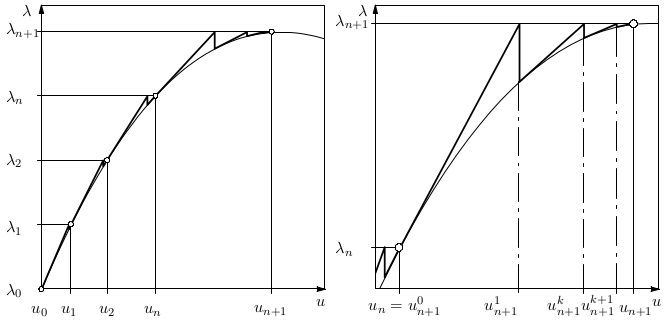
\includegraphics[scale=0.6]{Figure2/Chap3/load control and pure Newton-Raphson.png}
    \caption{Combination of load control and pure Newton-Raphson method}
    \label{fig:7.5}
\end{figure}

\begin{figure}[H]
    \centering
    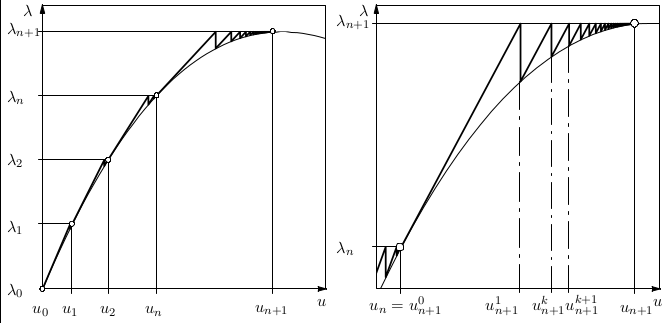
\includegraphics[scale=0.6]{Figure2/Chap3/load control and modified Newton-Raphson.png}
    \caption{Combination of load control and modified Newton-Raphson iteration}
    \label{fig:7.6}
\end{figure}